\subsection{特殊な関手}\label{chap-6.3-unique-functor}
  ある圏$\cat{C}$の二対象$A,B$の射集合$\arset{C}{A}{B}$は$A,B$で添字付けられていて、射写像$\arset{C}{A}{f}$も射で添字付けられているように見える。実際にこの操作は関手であるが、この段階ではこの操作を関手で表すことが難しい。そのため前提知識として双関手、反変関手を定義し見ていく。\\
	最初に対象や射を二つ取るような2変数関数のような関手、双関手について考える。
	\begin{define}[双関手]\label{def-bifunctor}
		積圏からの関手、つまり$\functor{F}{A\times B}{C}$となるような関手を\textbf{双関手}とする。

		また積圏の任意の対象$[A,B]$に対し、\[F(\pcobj{A,B})=F(A,B)\]と略記する。
		さらに積圏の射$\mor{\pcobj{f,id_B}}{\pcobj{A,B}}{\pcobj{A,B'}}$において\[F(\pcobj{f,id_B})=F(f,B)\]と表記する。
	\end{define}
	圏$\cat{A}$の射$f$と圏$\cat{B}$の射$g$がどのように圏$\cat{C}$に写されるのかを以下の可換図式で確認してほしい。等式としては示さないが、右の図式は関手の合成の保存によって可換になることに注意してほしい。
	\begin{center}
		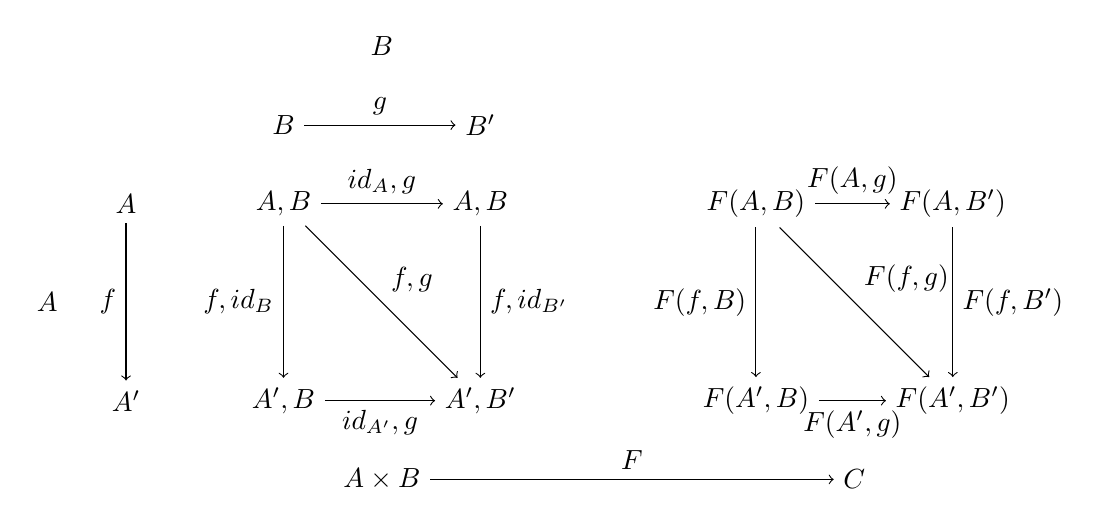
\begin{tikzpicture}[auto]
			\node (a) at (0, 0) {$A$};
			\node (a') at (0, -2.5) {$A'$};
			\node (b) at (2, 1) {$B$};
			\node (b') at (4.5, 1) {$B'$};
			\node (ab) at (2, 0) {$\pcobj{A,B}$};
			\node (a'b) at (2, -2.5) {$\pcobj{A',B}$};
			\node (ab') at (4.5, 0) {$\pcobj{A,B}$};
			\node (a'b') at (4.5, -2.5) {$\pcobj{A',B'}$};

			\node (fab) at (8, 0) {$F(A,B)$};
			\node (fa'b) at (8, -2.5) {$F(A',B)$};
			\node (fab') at (10.5, 0) {$F(A,B')$};
			\node (fa'b') at (10.5, -2.5) {$F(A',B')$};

			\node (cata) at (-1, -1.25) {$\cat{A}$};
			\node (catb) at (3.25, 2) {$\cat{B}$};
			\node (catab) at (3.25, -3.5) {$\cat{A\times B}$};
			\node (catc) at (9.25, -3.5) {$\cat{C}$};

			\draw[->] (a) to node[swap]{$f$}(a');
			\draw[->] (b) to node{$g$}(b');
			\draw[->] (ab) to node[swap]{$\pcobj{f,id_B}$}(a'b);
			\draw[->] (ab') to node{$\pcobj{f,id_{B'}}$}(a'b');
			\draw[->] (ab) to node{$\pcobj{id_A,g}$}(ab');
			\draw[->] (a'b) to node[swap]{$\pcobj{id_{A'},g}$}(a'b');
			\draw[->] (ab) to node{$\pcobj{f,g}$}(a'b');

			\draw[->] (fab) to node[swap]{$F(f,B)$}(fa'b);
			\draw[->] (fab') to node{$F(f,B')$}(fa'b');
			\draw[->] (fab) to node{$F(A,g)$}(fab');
			\draw[->] (fa'b) to node[swap]{$F(A',g)$}(fa'b');
			\draw[->] (fab) to node{$F(f,g)$}(fa'b');
			\draw[->] (catab) to node{$F$}(catc);
		\end{tikzpicture}
	\end{center}
  双関手は関手を量化とみなすのであれば、複数の圏のそれぞれの対象、射で同時に量化していると考えられる。\\
	次に双関手の例として積関手$\functor{-\times B}{C}{C}$を双関手に拡張しようと思う。
	\begin{define}[双積関手]\label{def-biproduct-functor}
		積を持つ圏$\cat{C}$上の\textbf{双積関手}$\functor{-\times -}{C\times C}{C}$を以下の写像で定義する。
		\begin{quote}
			\begin{mydescription}
				\item[対象関数] 対象関数を積圏$\cat{C\times C}$の任意の対象$\pcobj{A,B}$に対して\[(-\times -)(A,B)=A\times B\]と定義する。
				\item[射関数] 二対象$\pcobj{A,B},\pcobj{A',B'}$に対する射関数を任意の射$\mor{\pcobj{f,g}}{\pcobj{A,B}}{\pcobj{A',B'}}$に対して\[(-\times -)_{\pcobj{A,B},\pcobj{A',B'}}(f,g)=f\times g\]と定義する。
				\begin{center}
					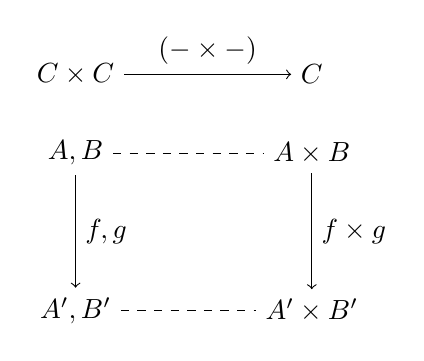
\begin{tikzpicture}[auto]
						\node (ab) at (0, 0) {$\pcobj{A,B}$};
						\node (a'b') at (0, -2) {$\pcobj{A',B'}$};
						\node (pab) at (3, 0) {$A\times B$};
						\node (pa'b') at (3, -2) {$A'\times B'$};
						\node (catcc) at (0, 1) {$\cat{C\times C}$};
						\node (catc) at (3, 1) {$\cat{C}$};
						\draw[-,dashed] (ab) to (pab);
						\draw[-,dashed] (a'b') to (pa'b');
						\draw[->] (ab) to node{$\pcobj{f,g}$}(a'b');
						\draw[->] (pab) to node{$f\times g$}(pa'b');
						\draw[->] (catcc) to node{$(-\times-)$}(catc);
					\end{tikzpicture}
				\end{center}

				\item[恒等射の保存] $(-\times -)(id_{\pcobj{A,B}})=id_{(-\times-)(A,B)}$を示せばよい。
				\begin{align*}
					(-\times -)(id_{\pcobj{A,B}})&=id_A\times id_B&\text{(射関数の定義)}\\
					&=\pcobj{id_A\circ\pi_A,id_B\circ\pi_B}&\text{(射の積の定義)}\\
					&=id_{A\times B}&\text{(射影射の対)}\\
					&=id_{(-\times-)(A,B)}&\text{(対象関数の定義)}
				\end{align*}
				よって恒等射を保つ。
				\item[射の合成の保存] $(-\times -)(f',g')\circ(-\times-)(f,g)=(-\times-)(\pcobj{f',g'}\circ\pcobj{f,g})$を示せばよい。
				\begin{align*}
					(-\times -)(f',g')\circ(-\times-)(f,g)&=(f'\times g')\circ(f\times g)&\text{(射関数の定義)}\\
					&=(f'\circ f)\times(g'\circ g)&\text{(積と合成の交換)}\\
					&=(-\times-)(f'\circ f,g'\circ g)&\text{(射関数の定義)}\\
					&=(-\times-)(\pcobj{f'\circ f,g'\circ g})\\
					&=(-\times-)(\pcobj{f',g'}\circ\pcobj{f,g})&\text{(積圏の射の合成の定義)}
				\end{align*}
				よって射の合成を保つ。
			\end{mydescription}
		\end{quote}
	\end{define}
	対象の積と圏の積が紛らわしいが、まず圏の積の対象$\pcobj{A,B}$は圏$\cat{C}$の$A$と$B$の積が存在しなくとも定義することができ、その点で対象の積$A\times B$より一般的な概念だと考えられる。よってイメージとしては圏$\cat{C}$の外側$\cat{C\times C}$で定義した対象の積もどき$[A,B]$を圏$\cat{C}$に積対象$A\times B$として挿入する操作が関手$(-\times-)$と考えられる。ただし、双積関手で写された対象が積の普遍性を満たすかどうかは現段階では説明できない。

	また以前に圏$\cat{C}$の射の積と積圏$\cat{C\times C}$の射の振る舞いが似ていることについて述べたが、実際に関手として二つの射の関係性を示すことができた。

  次に反変関手を定義するのであるが、これは厳密には関手ではない。しかし関手として扱う方法があり、そのために圏の双対について説明する。
	\begin{define}[双対圏]\label{def-opposite-category}
		ある圏$\cat{C}$に対する\textbf{双対圏}$\cat{C}^{op}$を以下の要素で定義する。
		\begin{quote}
			\begin{mydescription}
				\item[対象] $\obj{C^{op}}=\obj{C}$とする。

				また圏$\cat{C}$の対象$A$に対応する双対圏$\cat{C^{op}}$の対象も$A$であるが、$\cat{C^{op}}$の対象は$A^{op}$として表記上区別する。
				\item[射] 任意の二対象$A^{op}, B^{op}$に対して射集合を\[\arset{C^{op}}{B^{op}}{A^{op}}=\arset{C}{A}{B}\]と定義する。
				同様に射$\mor{f}{A}{B}$に対応する射を表記上$\mor{f^{op}}{B^{op}}{A^{op}}$とする。
				圏$\cat{C}$と双対圏$\cat{C^{op}}$では射の向きが入れ替わっていることに注意してほしい。
				\begin{center}
					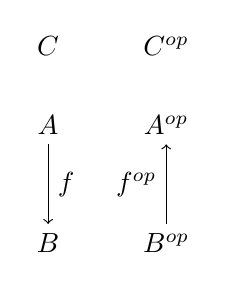
\begin{tikzpicture}[auto]
						\node (a) at (0, 0) {$A$};
						\node (b) at (0, -1.5) {$B$};
						\node (fa) at (1.5, 0) {$A^{op}$};
						\node (fb) at (1.5, -1.5) {$B^{op}$};
						\node (catc) at (0, 1) {$\cat{C}$};
						\node (catd) at (1.5, 1) {$\cat{C^{op}}$};
						\draw[->] (a) to node{$f$}(b);
						\draw[->] (fb) to node{$f^{op}$}(fa);
					\end{tikzpicture}
				\end{center}
				\item[射の合成] 圏$\cat{C}$の射$\mor{f}{A}{B}$、$\mor{g}{B}{C}$の合成射$\mor{g\circ f}{A}{C}$に対して、双対圏$\cat{C}^{op}$の射$\mor{f^{op}}{B^{op}}{A^{op}}$、$\mor{g^{op}}{C^{op}}{B^{op}}$の合成射を
				\[\mor{(g\circ f)^{op}=f^{op}\circ g^{op}}{C^{op}}{A^{op}}\]
				と定義する。
				圏$\cat{C}$と$\cat{C}^{op}$では射の合成の順序が入れ替わっていることに注意してほしい。
				\begin{center}
					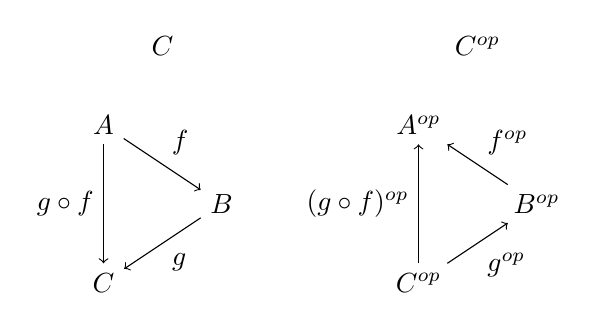
\begin{tikzpicture}[auto]
						\node (a) at (0, 0) {$A$};
						\node (b) at (1.5, -1) {$B$};
						\node (c) at (0, -2) {$C$};
						\node (fa) at (4, 0) {$A^{op}$};
						\node (fb) at (5.5, -1) {$B^{op}$};
						\node (fc) at (4, -2) {$C^{op}$};
						\node (catc) at (0.75, 1) {$\cat{C}$};
						\node (catd) at (4.75, 1) {$\cat{C^{op}}$};
						\draw[->] (a) to node{$f$}(b);
						\draw[->] (b) to node{$g$}(c);
						\draw[->] (a) to node[swap]{$g\circ f$}(c);
						\draw[->] (fb) to node[swap]{$f^{op}$}(fa);
						\draw[->] (fc) to node[swap]{$g^{op}$}(fb);
						\draw[->] (fc) to node{$(g\circ f)^{op}$}(fa);
					\end{tikzpicture}
				\end{center}
				\item[恒等射の存在]圏$\cat{C}$の任意の恒等射$\mor{id_A}{A}{A}$に対して、双対圏$\cat{C}^{op}$の恒等射を\[\mor{(id_A)^{op}=id_{A^{op}}}{A^{op}}{A^{op}}\]と定義する。
				\item[結合律] 合成可能な任意の射$f^{op},g^{op},h^{op}$において、
				\begin{align*}
					(f^{op}\circ g^{op})\circ h^{op}&=(g\circ f)^{op}\circ h^{op}\\
					&=(h\circ(g\circ f))^{op}\\
					&=((h\circ g)\circ f)^{op}\\
					&=f^{op}\circ (h\circ g)^{op}\\
					&=f^{op}\circ (g^{op}\circ h^{op})
				\end{align*}
				となるので結合律を満たす。
				\item[単位元律]任意の恒等射$id_{A^{op}}$、任意の射$\mor{f^{op}}{X^{op}}{A^{op}}$、$\mor{g^{op}}{A^{op}}{Y^{op}}$に対し$id_{A^{op}}\circ f^{op}=f^{op}$、$g^{op}\circ id_{A^{op}}=g^{op}$を示せばよい。
				\begin{align*}
					id_{A^{op}}\circ f^{op}&={id_A}^{op}\circ f^{op}&\text{(双対圏の恒等射の定義)}\\
					&=(f\circ id_A)^{op}&\text{(双対圏の射の合成の定義)}\\
					&=f^{op}&\text{(単位元律)}\\
					g^{op}\circ id_{A^{op}}&=g^{op}\circ {id_A}^{op}&\text{(双対圏の恒等射の定義)}\\
					&=(id_A\circ g)^{op}&\text{(双対圏の射の合成の定義)}\\
					&=g^{op}&\text{(単位元律)}\\
				\end{align*}
				よって単位元律を見たす。
			\end{mydescription}
		\end{quote}
	\end{define}
	圏の射をすべて反転した圏が双対圏であったが、圏から圏への関手から、双対圏から双対圏への関手を構成することができる。記述がややこしくなってしまったが、定義としては反転した射を反転した射に写すだけである。
	\begin{define}[双対関手]\label{def-opposite-functor}
		ある圏$\cat{C,D}$に対する双対圏$\cat{C}^{op},\cat{D}^{op}$と関手$\functor{F}{C}{D}$に対して、双対関手$\functor{F^{op}}{C^{op}}{D^{op}}$を以下の要素で定義する。
		\begin{quote}
			\begin{mydescription}
				\item[対象関数]対象関数$\mor{F^{op}}{C^{op}}{D^{op}}$を任意の対象$A^{op}$に対して
				\[F^{op}(A^{op})=(FA)^{op}\]と定義する。
				
				\item[射関数]対象関数と同様に、射関数\[\mor{{F^{op}}_{A^{op},B^{op}}}{\arset{C^{op}}{A^{op}}{B^{op}}}{\arset{D^{op}}{(FA)^{op}}{(FB)^{op}}}\]を任意の射$\mor{f}{A^{op}}{B^{op}}$に対して
				\[F^{op}(f^{op})=(Ff)^{op}\]と定義する。

				\begin{center}
					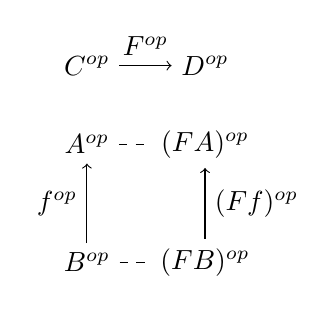
\begin{tikzpicture}[auto]
						\node (a) at (0, 0) {$A^{op}$};
						\node (b) at (0, -1.5) {$B^{op}$};
						\node (fa) at (1.5, 0) {$(FA)^{op}$};
						\node (fb) at (1.5, -1.5) {$(FB)^{op}$};
						\node (catc) at (0, 1) {$\cat{C^{op}}$};
						\node (catd) at (1.5, 1) {$\cat{D^{op}}$};
						\draw[-,dashed] (a) to (fa);
						\draw[-,dashed] (b) to (fb);
						\draw[->] (b) to node{$f^{op}$}(a);
						\draw[->] (fb) to node[swap]{$(Ff)^{op}$}(fa);
						\draw[->] (catc) to node{$F^{op}$}(catd);
					\end{tikzpicture}
					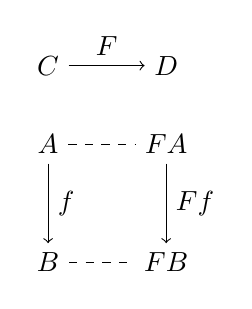
\begin{tikzpicture}[auto]
						\node (a) at (0, 0) {$A$};
						\node (b) at (0, -1.5) {$B$};
						\node (fa) at (1.5, 0) {$FA$};
						\node (fb) at (1.5, -1.5) {$FB$};
						\node (catc) at (0, 1) {$\cat{C}$};
						\node (catd) at (1.5, 1) {$\cat{D}$};
						\draw[-,dashed] (a) to (fa);
						\draw[-,dashed] (b) to (fb);
						\draw[->] (a) to node{$f$}(b);
						\draw[->] (fa) to node{$Ff$}(fb);
						\draw[->] (catc) to node{$F$}(catd);
					\end{tikzpicture}
				\end{center}
				\item[恒等射の保存]元の関手$F$の恒等射の保存に還元して$F^{op}(id_{A^{op}})=id_{(FA)^{op}}$を示す
				\begin{align*}
					F^{op}(id_{A^{op}})&=F^{op}(id_A)^{op}&\text{(双対圏の恒等射の定義)}\\
					&=(F(id_A))^{op}&\text{(双対関手の射関数の定義)}\\
					&=(id_{FA})^{op}&\text{($F$の恒等者の保存)}\\
					&=id_{(FA)^{op}}&\text{(双対圏の恒等射の定義)}
				\end{align*}
				
				\item[射の合成の保存]同様に元の関手の合成の保存に還元して\[F^{op}(f^{op}\circ g^{op})=F^{op}f^{op}\circ F^{op}g^{op}\]を示す。
				\begin{align*}
					F^{op}(f^{op}\circ g^{op})&= F^{op}(g\circ f)^{op}&\text{(双対圏の射の合成)}\\
					&=(F(g\circ f))^{op}&\text{(双対関手の射関数の定義)}\\
					&=(Fg\circ Ff)^{op}&\text{($F$の射の合成の保存)}\\
					&=(Fg)^{op}\circ (Ff)^{op}&\text{(双対圏の射の合成)}\\
					&=F^{op}f^{op}\circ F^{op}g^{op}&\text{(双対関手の射関数の定義)}
				\end{align*}
			\end{mydescription}
		\end{quote}
	\end{define}

	双対関手では反転した射を反転したまま写した。次に定義する反変関手では通常の射を反転した射に写すような捻れた操作を考える。この捻れによって関手の定義とは異なるものになることを注意してほしい。
	\begin{define}[反変関手]\label{def-contravariant-functor}
		圏$\cat{C}$から圏$\cat{D}$への\textbf{反変関手}と呼ばれる圏の間の写像$\functor{F}{C}{D}$を以下の写像と公理で定義する。
		\begin{quote}
			\begin{mydescription}
				\item[対象関数] $\cat{C}$の対象$A$に$\cat{D}$の対象$FA$を割り当てる対象関数\[\mor{F}{\obj{C}}{\obj{D}}\]を持つ必要がある。\\
				これは通常の関手と同じである。
				\item[射関数] $\cat{C}$の任意の各対象$A,B$において射$\mor{f}{A}{B}$に圏$\cat{D}$の射$\mor{Ff}{FB}{FA}$を割り当てる射関数\[\mor{F_{A,B}}{\arset{C}{A}{B}}{\arset{D}{FB}{FA}}\]を持つ必要がある。射の向きが変わってしまうが、関手と同様にこれも同様に対象$A,B$に対してそれぞれ存在する射関数$F_{A,B}$を総称して$F$と呼ぶことにする。
				\begin{center}
					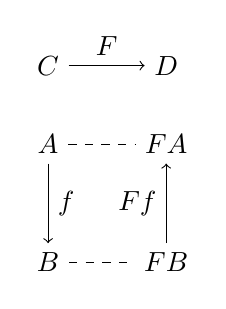
\begin{tikzpicture}[auto]
						\node (a) at (0, 0) {$A$};
						\node (b) at (0, -1.5) {$B$};
						\node (fa) at (1.5, 0) {$FA$};
						\node (fb) at (1.5, -1.5) {$FB$};
						\node (catc) at (0, 1) {$\cat{C}$};
						\node (catd) at (1.5, 1) {$\cat{D}$};
						\draw[-,dashed] (a) to (fa);
						\draw[-,dashed] (b) to (fb);
						\draw[->] (a) to node{$f$}(b);
						\draw[->] (fb) to node{$Ff$}(fa);
						\draw[->] (catc) to node{$F$}(catd);
					\end{tikzpicture}
				\end{center}
				双対圏を取る操作と同じように、射を写すときは射の向きを逆にする。
				\item[恒等射の保存] $F(id_A)=id_{FA}$が任意の恒等射で成り立つ。
				\item[射の合成の保存] 合成可能な任意の二射$f,g$において\[F(g\circ f)=Ff\circ Fg\]が成り立つ。

				\begin{center}
					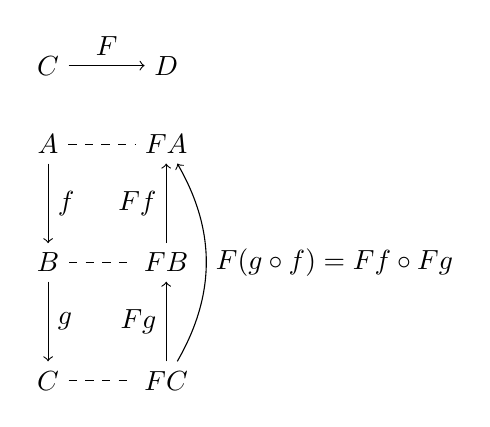
\begin{tikzpicture}[auto]
						\node (a) at (0, 0) {$A$};
						\node (b) at (0, -1.5) {$B$};
						\node (c) at (0, -3) {$C$};
						\node (fa) at (1.5, 0) {$FA$};
						\node (fb) at (1.5, -1.5) {$FB$};
						\node (fc) at (1.5, -3) {$FC$};
						\node (catc) at (0, 1) {$\cat{C}$};
						\node (catd) at (1.5, 1) {$\cat{D}$};
						\draw[-,dashed] (a) to (fa);
						\draw[-,dashed] (b) to (fb);
						\draw[-,dashed] (c) to (fc);
						\draw[->] (a) to node{$f$}(b);
						\draw[->] (b) to node{$g$}(c);
						\draw[->] (fb) to node{$Ff$}(fa);
						\draw[->] (fc) to node{$Fg$}(fb);
						\draw[->,bend right = 30] (fc) to node[swap]{$F(g\circ f)=Ff\circ Fg$}(fa);
						\draw[->] (catc) to node{$F$}(catd);
					\end{tikzpicture}
				\end{center}
				双対圏の射の合成と同じように、合成射を写すときは合成の順序を逆にして写す。
			\end{mydescription}
		\end{quote}
	\end{define}
	反変関手は関手とついているが、双対関手とは違い以前定義した関手の性質を満たさず、関手とはならない。そのため区別が必要な場合、一般の関手を\textbf{共変関手}と呼ぶことにする。\\
	また反変関手$\functor{F}{C}{D}$は双対圏によって共変関手$\functor{F}{C^{op}}{D}$とみなせることが図式から分かる。
		\begin{center}
			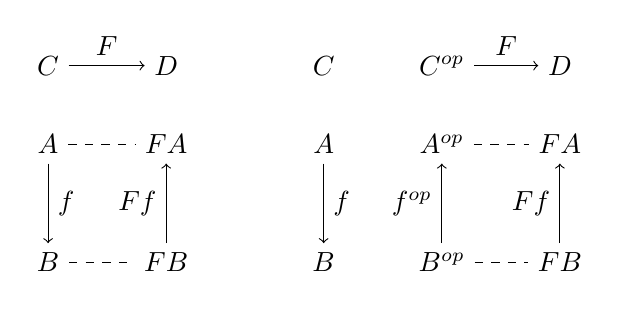
\begin{tikzpicture}[auto]
				\node (a) at (0, 0) {$A$};
				\node (b) at (0, -1.5) {$B$};
				\node (fa) at (1.5, 0) {$FA$};
				\node (fb) at (1.5, -1.5) {$FB$};
				\node (catc) at (0, 1) {$\cat{C}$};
				\node (catd) at (1.5, 1) {$\cat{D}$};
				\draw[-,dashed] (a) to (fa);
				\draw[-,dashed] (b) to (fb);
				\draw[->] (a) to node{$f$}(b);
				\draw[->] (fb) to node{$Ff$}(fa);
				\draw[->] (catc) to node{$F$}(catd);

				\node (a) at (3.5, 0) {$A$};
				\node (b) at (3.5, -1.5) {$B$};
				\node (aop) at (5, 0) {$A^{op}$};
				\node (bop) at (5, -1.5) {$B^{op}$};
				\node (fa) at (6.5, 0) {$FA$};
				\node (fb) at (6.5, -1.5) {$FB$};
				\node (catcop) at (3.5, 1) {$\cat{C}$};
				\node (catc) at (5, 1) {$\cat{C^{op}}$};
				\node (catd) at (6.5, 1) {$\cat{D}$};
				\draw[-,dashed] (aop) to (fa);
				\draw[-,dashed] (bop) to (fb);
				\draw[->] (bop) to node{$f^{op}$}(aop);
				\draw[->] (a) to node{$f$}(b);
				\draw[->] (fb) to node{$Ff$}(fa);
				\draw[->] (catc) to node{$F$}(catd);
			\end{tikzpicture}
		\end{center}
	